\nonumchapter{Экспериментальные результаты}
\section{Исследуемые образцы}

В данной работе были исследованы образцы, представляющие собой пары параллельных наностержней из золота, расположенных на подложке из плавленного кварца. Ансамбли из наностержней были изготовлены с помощью  электронно-лучевой литографии коллегами из Парижского института фундаментальной электроники (Institut d'Electronique Fondamentale). Наноструктурированная поверхность с одинаковыми парами наностержней была площадью 100*100 мкм$ ^2 $, и на ней находилось приблизительно 10$ ^4 $ пар наностержней --- димеров. 
На рис.~\ref{img:sample} схематично показано расположение ансамблей димеров наностержней на одной подложке из плавленного кварца с толщиной 0.5 мм. В каждом ансамбле димеров все геометрические параметры наностержней были одинаковые, в то время как в различных ансамблях варьировалась длина наностержней и расстояние между ними. Длина наностержней составляла $ a = $ 100, 150, 200, 400, 500 нм, а расстояние между ними -- $ d = $ 100, 150, 250, 350, 450, 650 нм. Высота и ширина наностержней были фиксированы и равнялись 50 нм. Расстояние между ансамблями димеров составляло 850 мкм. 
\begin{figure}[!h]
\center{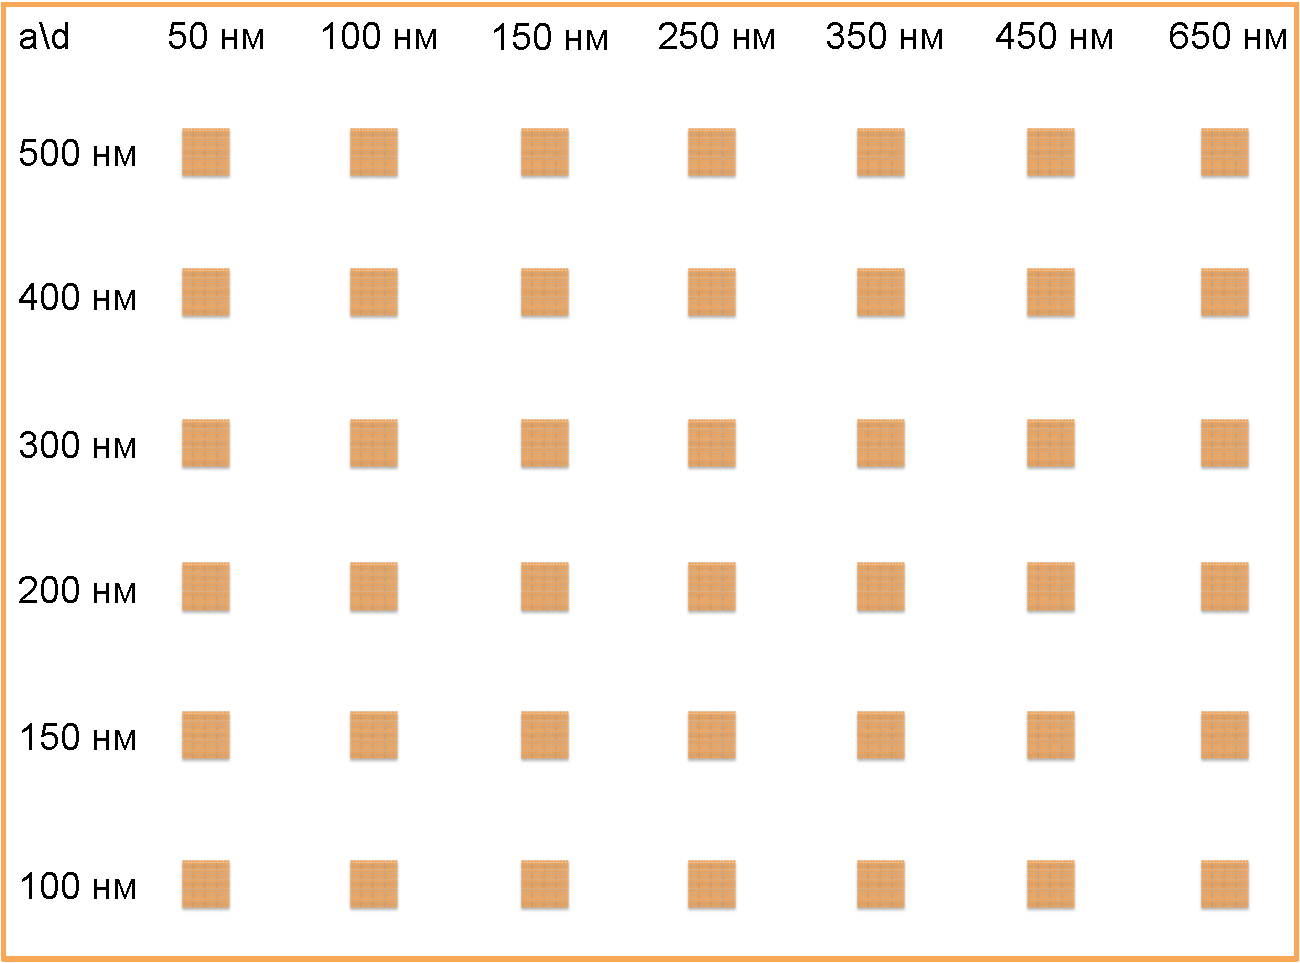
\includegraphics[width=10cm]{img/samples.pdf}}
\caption{Схематичное расположение ансамблей димеров золотых наностержней на подложке. В каждом из ансамблей фиксирована длина наностержней \textit{a} и расстояние \textit{d} между ними. Расстояние между ансамблями димеров составляла 850 мкм.}
\label{img:sample}
\end{figure}

Расстояние между димерами наностержней составляло 1 мкм, чтобы обеспечить отсутствие ближнепольного взаимодействия между димерами. На рис.~\ref{img:SEMsample} показано изображение одного из ансамблей димеров, полученного с помощью растрового электронного микроскопа.
\begin{figure}[!h]
\center{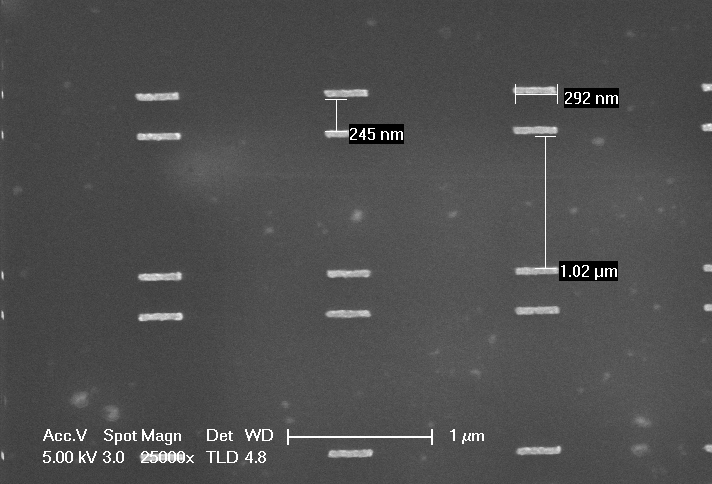
\includegraphics[width=10cm]{img/L300_d300_03.png}}
\caption{Изображение одного из исследуемых ансамблей димеров из золота, полученного с помощью растрового электронного микроскопа.}
\label{img:SEMsample}
\end{figure}
По изображениям с растрового электронного микроскопа также рассчитывалась погрешность в определении средней длины и ширины наностержней, составившая не более 3 нм и 1 нм, соответственно.

% Здесь секция для комментариев
% Все предложения в прошедшем  времени? 